\documentclass[10pt,a4paper]{article}
\usepackage[utf8]{inputenc}
\usepackage{amsmath}
\usepackage{amsfonts}
\usepackage{amssymb}
\usepackage{german}
\usepackage{fancyhdr}
\usepackage{graphicx}
\usepackage{geometry}
\usepackage{color}
\usepackage[usenames,dvipsnames,table]{xcolor}
\usepackage{DejaVuSans}
\usepackage[T1]{fontenc}
\usepackage[absolute]{textpos}

\fancypagestyle{lscape}{% 
\fancyhf{} % clear all header and footer fields 
\fancyfoot[LE]{%
\begin{textblock}{20}(1,5){\rotatebox{90}{\leftmark}}\end{textblock}
\begin{textblock}{1}(13,10.5){\rotatebox{90}{\thepage}}\end{textblock}}
\fancyfoot[LO] {%
\begin{textblock}{1}(14,2){\rotatebox{90}{Seite \thepage}}\end{textblock}
\begin{textblock}{20}(1,10){\rotatebox{90}{Projektplan - Verkehrsmodell-Fallstudien-Editor}}\end{textblock}
\begin{textblock}{20}(1,2){\rotatebox{90}{Dominik Heeb, Fabian Keller}}\end{textblock}
}
\renewcommand{\headrulewidth}{0pt} 
\renewcommand{\footrulewidth}{0pt}}

\usepackage{cite}
\usepackage{float}
\usepackage{wrapfig}
\usepackage{pdflscape}
\usepackage{rotating}
\usepackage[nottoc]{tocbibind}
\usepackage{epstopdf}
\usepackage{graphicx}
\usepackage{tabularx}
%\usepackage{floatrow}
\usepackage[T1]{fontenc}
\usepackage[utf8]{inputenc}
\usepackage{mathptmx}
\renewcommand{\rmdefault}{ptm}

\renewcommand*{\familydefault}{\sfdefault}
\geometry{verbose,a4paper,tmargin=35mm,bmargin=35mm,lmargin=25mm,rmargin=25mm}
\author{Dominik Heeb, Fabian Keller}
\title{Projektplan Bachelorarbeit}

\fancypagestyle{headings}{%
\fancyhead{}
\fancyhead[L]{Projektplan - Verkehrsmodell-Fallstudien-Editor}
\fancyhead[R]{Dominik Heeb, Fabian Keller}
\fancyfoot{}
\fancyfoot[R]{Seite \thepage}
\renewcommand{\headrulewidth}{1pt} }

\pagestyle{headings}
\begin{document}
\begin{titlepage}
	\begin{Huge}
		\begin{center}
				Projektplan \\Verkehrsmodell-Fallstudien-Editor\\[2.0cm]
		\end{center}
	\end{Huge}
	
	\begin{center}
		\begin{Large}
				von Dominik Heeb, Fabian Keller\\[1.0cm]
		\end{Large}
		\begin{large}
				Betreuer: Prof. Dr. Luc Bläser
		\end{large}
	\end{center}
\end{titlepage}

\newpage
\tableofcontents 
\newpage

\section{Management Abläufe}
\begin{flushleft}
	Diese Bachelorarbeit wird im Rahmen des Bachelor Studiums an der HSR durchgeführt welches bei erfolgreichem Abschluss mit 12 ECTS Punkten gewertet wird. Ein ECTS Punkt entspricht einem ungefähren Zeitaufwand von 25 bis 30 Stunden. Somit wird von jedem Teammitglied ein Zeitaufwand von ca. 300 bis 360 Stunden erwartet.
\end{flushleft}

\subsection{Zeitliche Planung}
	\begin{flushleft}
Der zeitliche Projektplan zeigt eine grobe zeitliche Übersicht über die gesamte Bachelorarbeit mit den einzelnen Iterationen und Meilensteinen.
	\end{flushleft}
	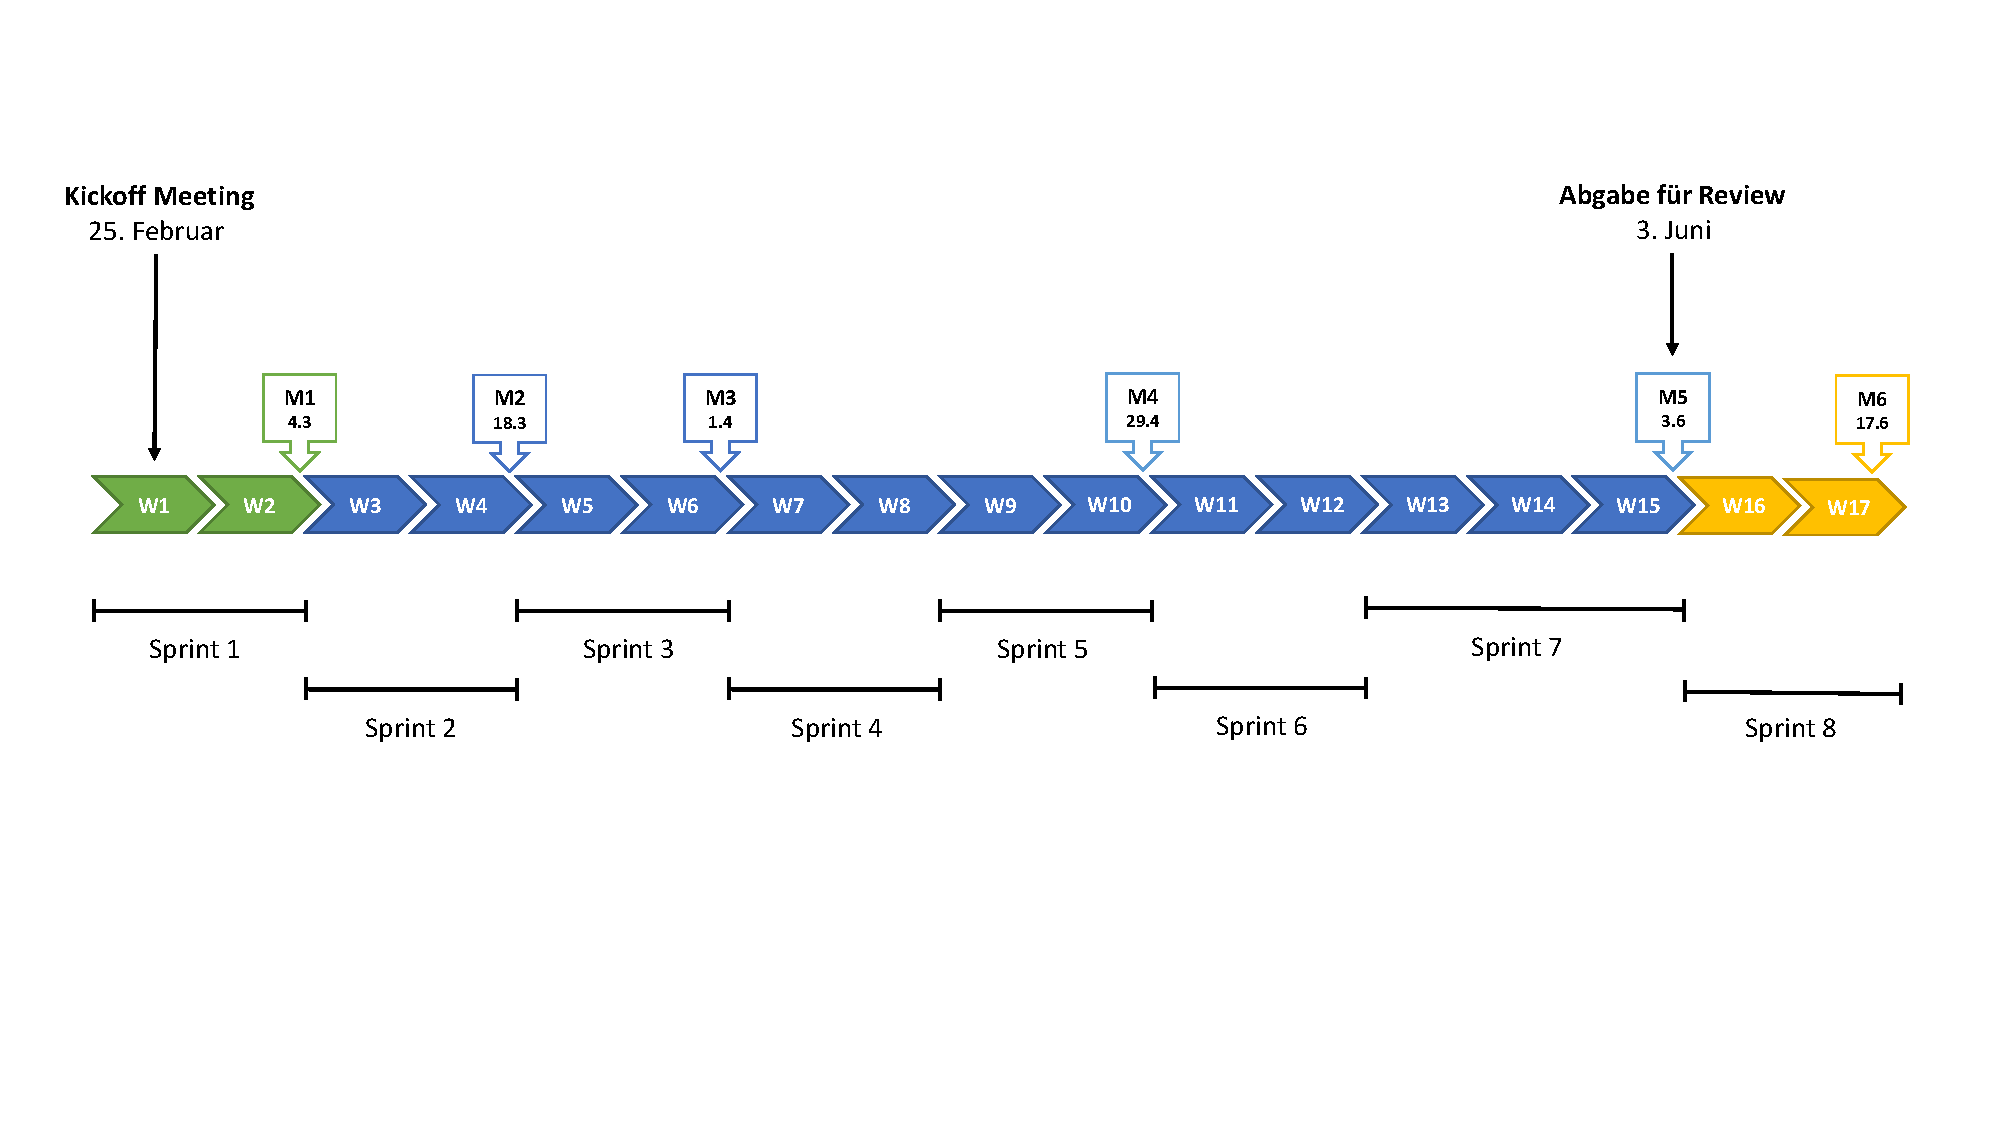
\includegraphics[width=17cm,height=7cm,trim=10mm 40mm 0mm 20mm, clip]{pictures/Meilensteinplan.pdf}

\subsection{Meilensteine}
\begin{flushleft}
Die einzelnen Meilensteine beinhalten folgende Ziele:
\end{flushleft}
\begin{tabular}{cl}
	\textcolor{ForestGreen}{\textbf{M1:}} & Projektplan erstellt, Infrastruktur fertig aufgebaut \\[0.2cm]
	\textcolor{NavyBlue}{\textbf{M2:}} & Prototyp v0.1: Anzeigen von Strassennetz in Online Map Editor \\[0.2cm]
	\textcolor{NavyBlue}{\textbf{M3:}} & Prototyp v0.2: Anzeigen von Parameter zu Strassen in Online Map Editor \\[0.2cm]
	\textcolor{NavyBlue}{\textbf{M4:}} & komplette Verkehrsdaten (Strassennetz, ÖV-Verkehsnetz, Parameter usw.) in Online Map-Editor darstellen\\[0.2cm]
	\textcolor{NavyBlue}{\textbf{M5:}} & Definierte Änderungen können an Verkehrsdaten in Online Map-Editor vorgenommen werden\\[0.2cm]
	\textcolor{Dandelion}{\textbf{M6:}} & Präsentation der Bachelorarbeit, Abgabe Bericht\\
\end{tabular}
\subsection{Besprechungen}
\begin{flushleft}
	Die Besprechung findet jede Woche am Donnerstag im Raum 1.167 um 14:00 Uhr statt. In dieser Besprechung wird der aktuelle Status der Bachelorarbeit und das weitere Vorgehen besprochen und offene Fragen geklärt.\\
Das Projektteam erstellt vor jeder Besprechung eine Traktandenliste und führt ein Sitzungsprotokoll. Dieses Protokoll wird anschliessend an den Betreuer und den Auftraggeber gesendet.
\end{flushleft}
\end{document}